\documentclass{article}
\usepackage{fancyhdr}
\usepackage{extramarks}
\usepackage{amsmath}
\usepackage{amsthm}
\usepackage{amsfonts}
\usepackage{graphicx}
\usepackage{cleveref}
\usepackage{hyperref}
\usepackage[backend=bibtex]{biblatex}


%
% Basic Document Settings
%
\setlength{\parindent}{1cm}
\topmargin=-0.45in
\evensidemargin=0in
\oddsidemargin=0in
\textwidth=6.5in
\textheight=9.0in
\headsep=0.25in

\linespread{1.1}

\pagestyle{fancy}
\rhead{\hmwkAuthorName}
\lhead{\hmwkClass\ : \hmwkTitle}
%\rhead{\firstxmark}
\lfoot{\lastxmark}
\cfoot{\thepage}

\renewcommand\headrulewidth{0.4pt}
\renewcommand\footrulewidth{0.4pt}

\setlength\parindent{0pt}

%
% Create Problem Sections
%

\newcommand{\enterProblemHeader}[1]{
    \nobreak\extramarks{}{Problem \arabic{#1} continued on next page\ldots}\nobreak{}
    \nobreak\extramarks{Problem \arabic{#1} (continued)}{Problem \arabic{#1} continued on next page\ldots}\nobreak{}
}

\newcommand{\exitProblemHeader}[1]{
    \nobreak\extramarks{Problem \arabic{#1} (continued)}{Problem \arabic{#1} continued on next page\ldots}\nobreak{}
    \stepcounter{#1}
    \nobreak\extramarks{Problem \arabic{#1}}{}\nobreak{}
}

\setcounter{secnumdepth}{0}
\newcounter{partCounter}
\newcounter{homeworkProblemCounter}
\setcounter{homeworkProblemCounter}{1}
\nobreak\extramarks{Problem \arabic{homeworkProblemCounter}}{}\nobreak{}

%
% Homework Problem Environment
%
% This environment takes an optional argument. When given, it will adjust the
% problem counter. This is useful for when the problems given for your
% assignment aren't sequential. See the last 3 problems of this template for an
% example.
%
\newenvironment{homeworkProblem}[1][-1]{
    \ifnum#1>0
        \setcounter{homeworkProblemCounter}{#1}
    \fi
    \section{Problem \arabic{homeworkProblemCounter}}
    \setcounter{partCounter}{1}
    \enterProblemHeader{homeworkProblemCounter}
}{
    \exitProblemHeader{homeworkProblemCounter}
}

%
% Homework Details
%   - Title
%   - Due date
%   - Class
%   - Section/Time
%   - Instructor
%   - Author
%

\newcommand{\hmwkTitle}{Assignment 4}
\newcommand{\hmwkDueDate}{September 21, 2015}
\newcommand{\hmwkClass}{Natural Language Understanding with Distributed
Representations}
\newcommand{\hmwkClassTime}{Section A}
\newcommand{\hmwkClassInstructor}{Professor Isaac Newton}
\newcommand{\hmwkAuthorName}{Felipe Ducau}
\newcommand{\hmwkNetID}{fnd212@nyu.edu}

%
% Title Page
%

\title{
    \vspace{2in}
    \textmd{\textbf{\hmwkClass}}\\
    \vspace{0.1in}
    \textmd{\textbf{\hmwkTitle}}\\     
    %\normalsize\vspace{0.1in}\small{Due\ on\ \hmwkDueDate}\\
%    \vspace{0.1in}\large{\textit{\hmwkClassInstructor\ \hmwkClassTime}}
    \vspace{3in}
}

\author{\textbf{\hmwkAuthorName}\\
		{\texttt{\hmwkNetID}}
}
\date{}

\renewcommand{\part}[1]{\textbf{\large Part \Alph{partCounter}}\stepcounter{partCounter}\\}

%
% Various Helper Commands
%

% Useful for algorithms
\newcommand{\alg}[1]{\textsc{\bfseries \footnotesize #1}}

% For derivatives
\newcommand{\deriv}[1]{\frac{\mathrm{d}}{\mathrm{d}x} (#1)}

% For partial derivatives
\newcommand{\pderiv}[2]{\frac{\partial}{\partial #1} (#2)}

% Integral dx
\newcommand{\dx}{\mathrm{d}x}

% Alias for the Solution section header
\newcommand{\solution}{\textbf{\large Solution}}

% Probability commands: Expectation, Variance, Covariance, Bias
\newcommand{\E}{\mathrm{E}}
\newcommand{\Var}{\mathrm{Var}}
\newcommand{\Cov}{\mathrm{Cov}}
\newcommand{\Bias}{\mathrm{Bias}}
\addbibresource{prop.bib}


\begin{document}

\maketitle

\pagebreak

{\section{1 Data Preparation}}

The data \footnote{https://github.com/neubig/nmt-tips} is composed of 11000 sentences in japanese with their corresponding translation in english. The training set contains 10000 sentences while both validation and test sets contain 500 sentences each. \\

Since the data is already in lowercase and the punctuation symbols already appear separated from other words by blank spaces, the only preprocessing used for the experiments of this assignment was to tokenize the words splitting them by spaces. \\

The size of the vocabulary in the english train set is 102207 words and in the japanese train set is 239126. From these words, to train our model we only keep the top 40000 words for each language. \\

The maximum longitude of sentence used along the experiments is 50, trimming those which were larger. The maximum sentence length along the train set is 66 for japanese sentences and 54 for english sentences The figure below shows the distribution of sentence lengths for each vocabulary.

\begin{center}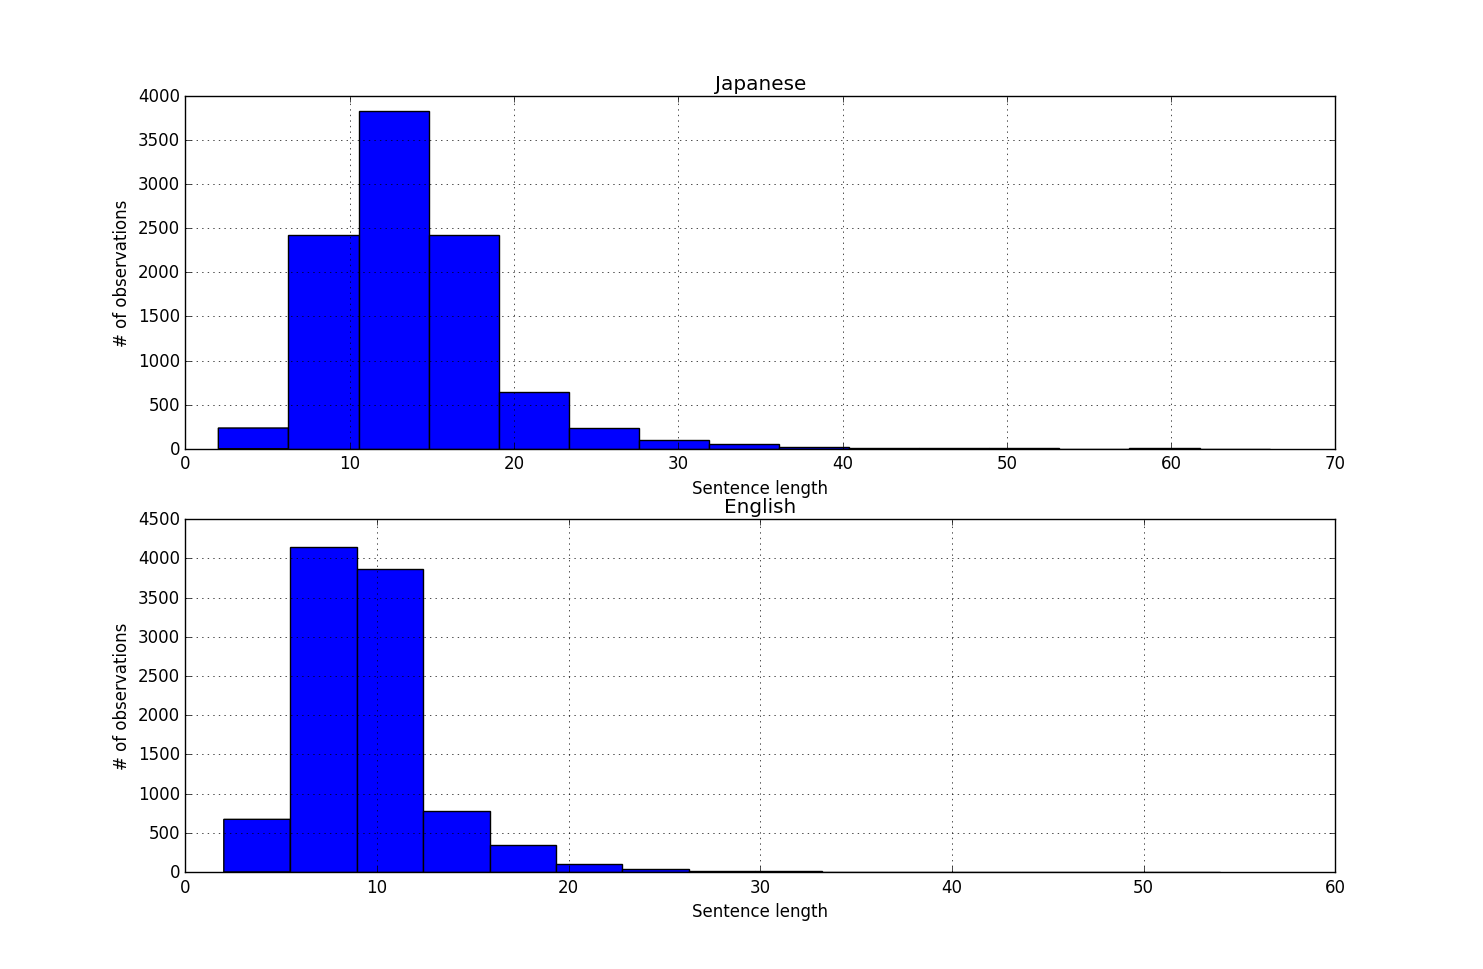
\includegraphics[scale=0.4]{sentence_len}\label{Sentence_Lengths}\end{center}\

{\section{2 Neural Machine Translation}}

The following parameters are common to both models implemented (Simple encoder-decoder and Attention-based NMT):\\

\begin{itemize}
    \item Word embedding dimension: 128.
    \item GRU context vector dimension: 256.
    \item Early stopping was impelemented with 10 of patience in the validation perplexity score. 
    \item Maximum longitude of a sentence: 50.
    \item Encoder RNN unit: GRU / Depth 1.
    \item Decoder RNN unit: GRU / Depth 1.
    \item Batch size: 100.
    \item Optimization method: Adadelta \cite{adadelta}.
    \item Initial learning: 0.01, then adaptive acording to Adadelta.
    \item Translation generation procedure: Greedy.
\end{itemize}

All the code for this assignment was implemented in Theano and it is based on parts of the code we are developing for our final project which is itself built upon \url{https://github.com/laulysta/nmt}. 


{\subsection{2.1 Simple Encoder-Decoder Model}}

The model used for this section was a basic Encoder-Decoder architecture with GRU units according to Cho et al 2014  \cite{cho_encdec} \\





{\subsection{2.1 Simple Encoder-Decoder Model}}

For this section, instead of using the output of the encoder as the input to the decoder, we implemented an attention mechanism in which the encoder looks at all the intermediate outputs of the encoder and create a weighted average of them according to its current input and memory state. \\

The implementation follows the one in \url{https://github.com/nyu-dl/dl4mt-tutorial} in which we use a bidirectional (forward and backward) encoder with a conditional GRU with attention mechanism for the decoder. \\


{\section{3 Results}}

Table \ref{results1} summarizes the results for the two different implementations. 

\begin{table}[h]
\centering

\begin{tabular}{cccccc}

Model                 &\vline &  Train Perplexity  & Validation Perplexity & Test BLEU \\
\hline
\hline
Encoder-Decoder       &\vline &  34.66                 & 88.52                   & 0.14 \\
Attention-based NMT   &\vline &  30.03                 & 75.19                   & 0.18  \\

\end{tabular}
\caption{Results.}
\label{results1}
\end{table}

The BLEU score in the table corresponds to the corpus level BLEU score \footnote{\url{http://www.nltk.org/_modules/nltk/translate/bleu_score.html}} which is smaller than the average of the BLEU score of the sentences. As expected, the basic model performs worth in terms of BLEU. The small value of the score is most probably consequence of the small size of the dataset. \\

The table below shows the training curves for both models. Even though the performance for the attention model is better overall, we note that the difference between the performance en train for both models decrease with the number of iterations. 

\begin{center}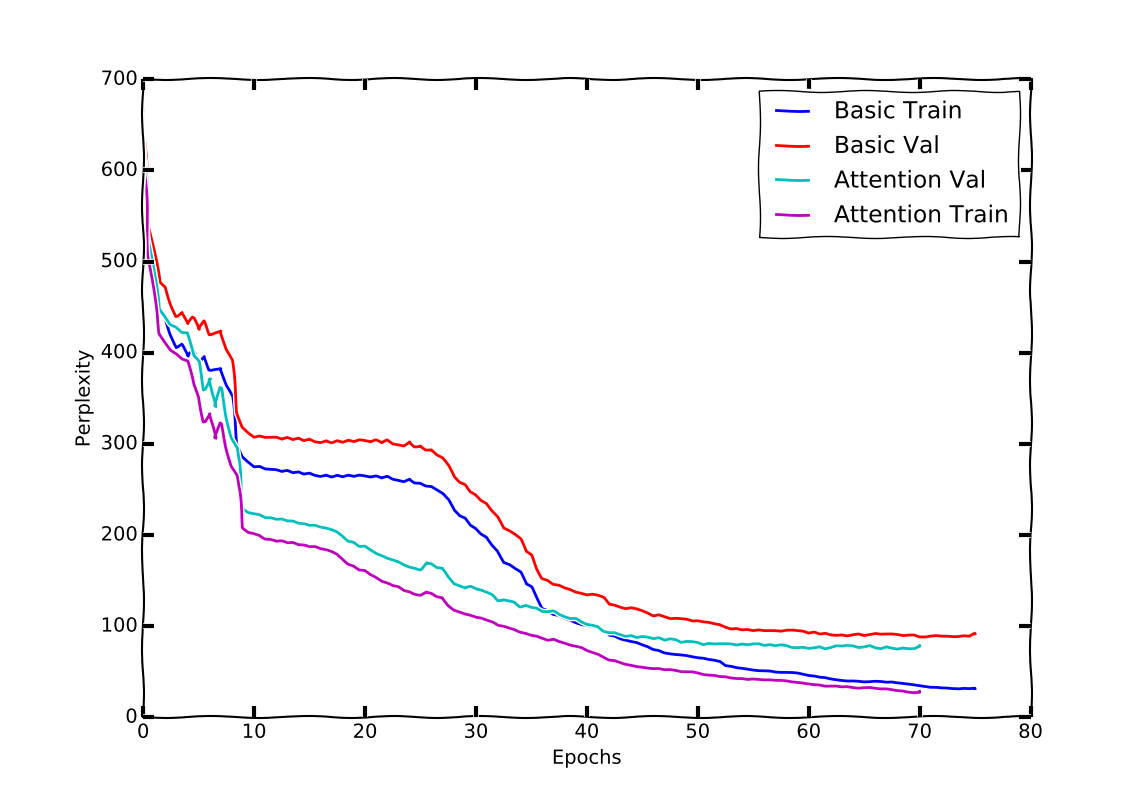
\includegraphics[scale=0.6]{results}\label{plotresults}\end{center}\


\printbibliography

\end{document}

